\part{Les objectifs de ce projet}
    \chapter{Les cas d'usage}
        \section{Objectifs : Qualité et productivité}

        Comme présenté précédemment (cf. \reffig{fig:processus_article}), la gestion de l'information produit est un processus lourd, avec des étapes de contrôle redondantes visant à assurer la qualité de la donnée.
        Un traitement automatique des documents mis à disposition permettrait de décharger les personnes qui interviennent dans le processus (fournisseurs, acheteurs, gestionnaires de référentiels, ingénieurs qualité) et de garantir une meilleure pertinence de l'information produit.

        \section{La préalimentation d'information}
        Une des manières de gagner en productivité et en qualité serait :
        \begin{itemize}
            \item de modifier l'interface homme machine de l'écran de saisie des données par le fournisseur, pour que le chargement des pièces jointes se fasse en premier
            \item d'interpréter le contenu des pièces jointes dès qu'elles sont chargées, pour alimenter les autres champs de saisie
            \item laisser ensuite au fournisseur la possibilité de compléter et corriger ces informations avant de les soumettre à Pomona
        \end{itemize} 
        Il est illusoire d'automatiser totalement la saisie et d'imaginer se passer d'une saisie complémentaire par le fournisseur.
        La mise en place de la GDSN (cf. section \mref{GDSN}), qui permet pourtant de faire transiter par EDI les données produit de manière standardisée et efficace, n'a pas permis de s'affranchir de cette tâche.
        Sous réserve d'avoir un outil suffisamment fiable, on pourrait faire gagner du temps aux fournisseurs et améliorer la qualité de l'information produit.
        Néanmoins, plusieurs freins existent à la mise en place 
        \begin{itemize}
            \item cela n'a d'intérêt que si le système est capable de produire de l'information structurée avec une fiabilité élevée (par exemple, 80\% de données correctes serait un minimum)
            \item cela entre en concurrence directe avec le système GDSN - avec la question de la manière de gérer les conflits entre les information issues de ce réseau et celles extraites des pièces jointes
            \item cela apporte l'essentiel de la valeur aux fournisseurs, et pas au groupe
        \end{itemize}

        \section{Le contrôle des informations transmises}

        Plus le taux de détection des erreurs est élevé, et plus les erreurs sont détectées tôt, mieux c'est : 
        \begin{itemize}
            \item la qualité des données s'en trouve évidemment améliorée
            \item le processus est plus court en temps, en évitant les aller-retours
            \item on décharge l'ensemble des acteurs, en limitant le nombre d'interventions de chacun, ainsi que la charge administrative de synchronisation de leurs actions             
        \end{itemize}
        Les différentes étapes possibles pour lesquelles effectuer un contrôle sont présentées à la \reffig{fig:processus_article_aide_ctrle}.

        \begin{figure}[htbp]
            \begin{center}
            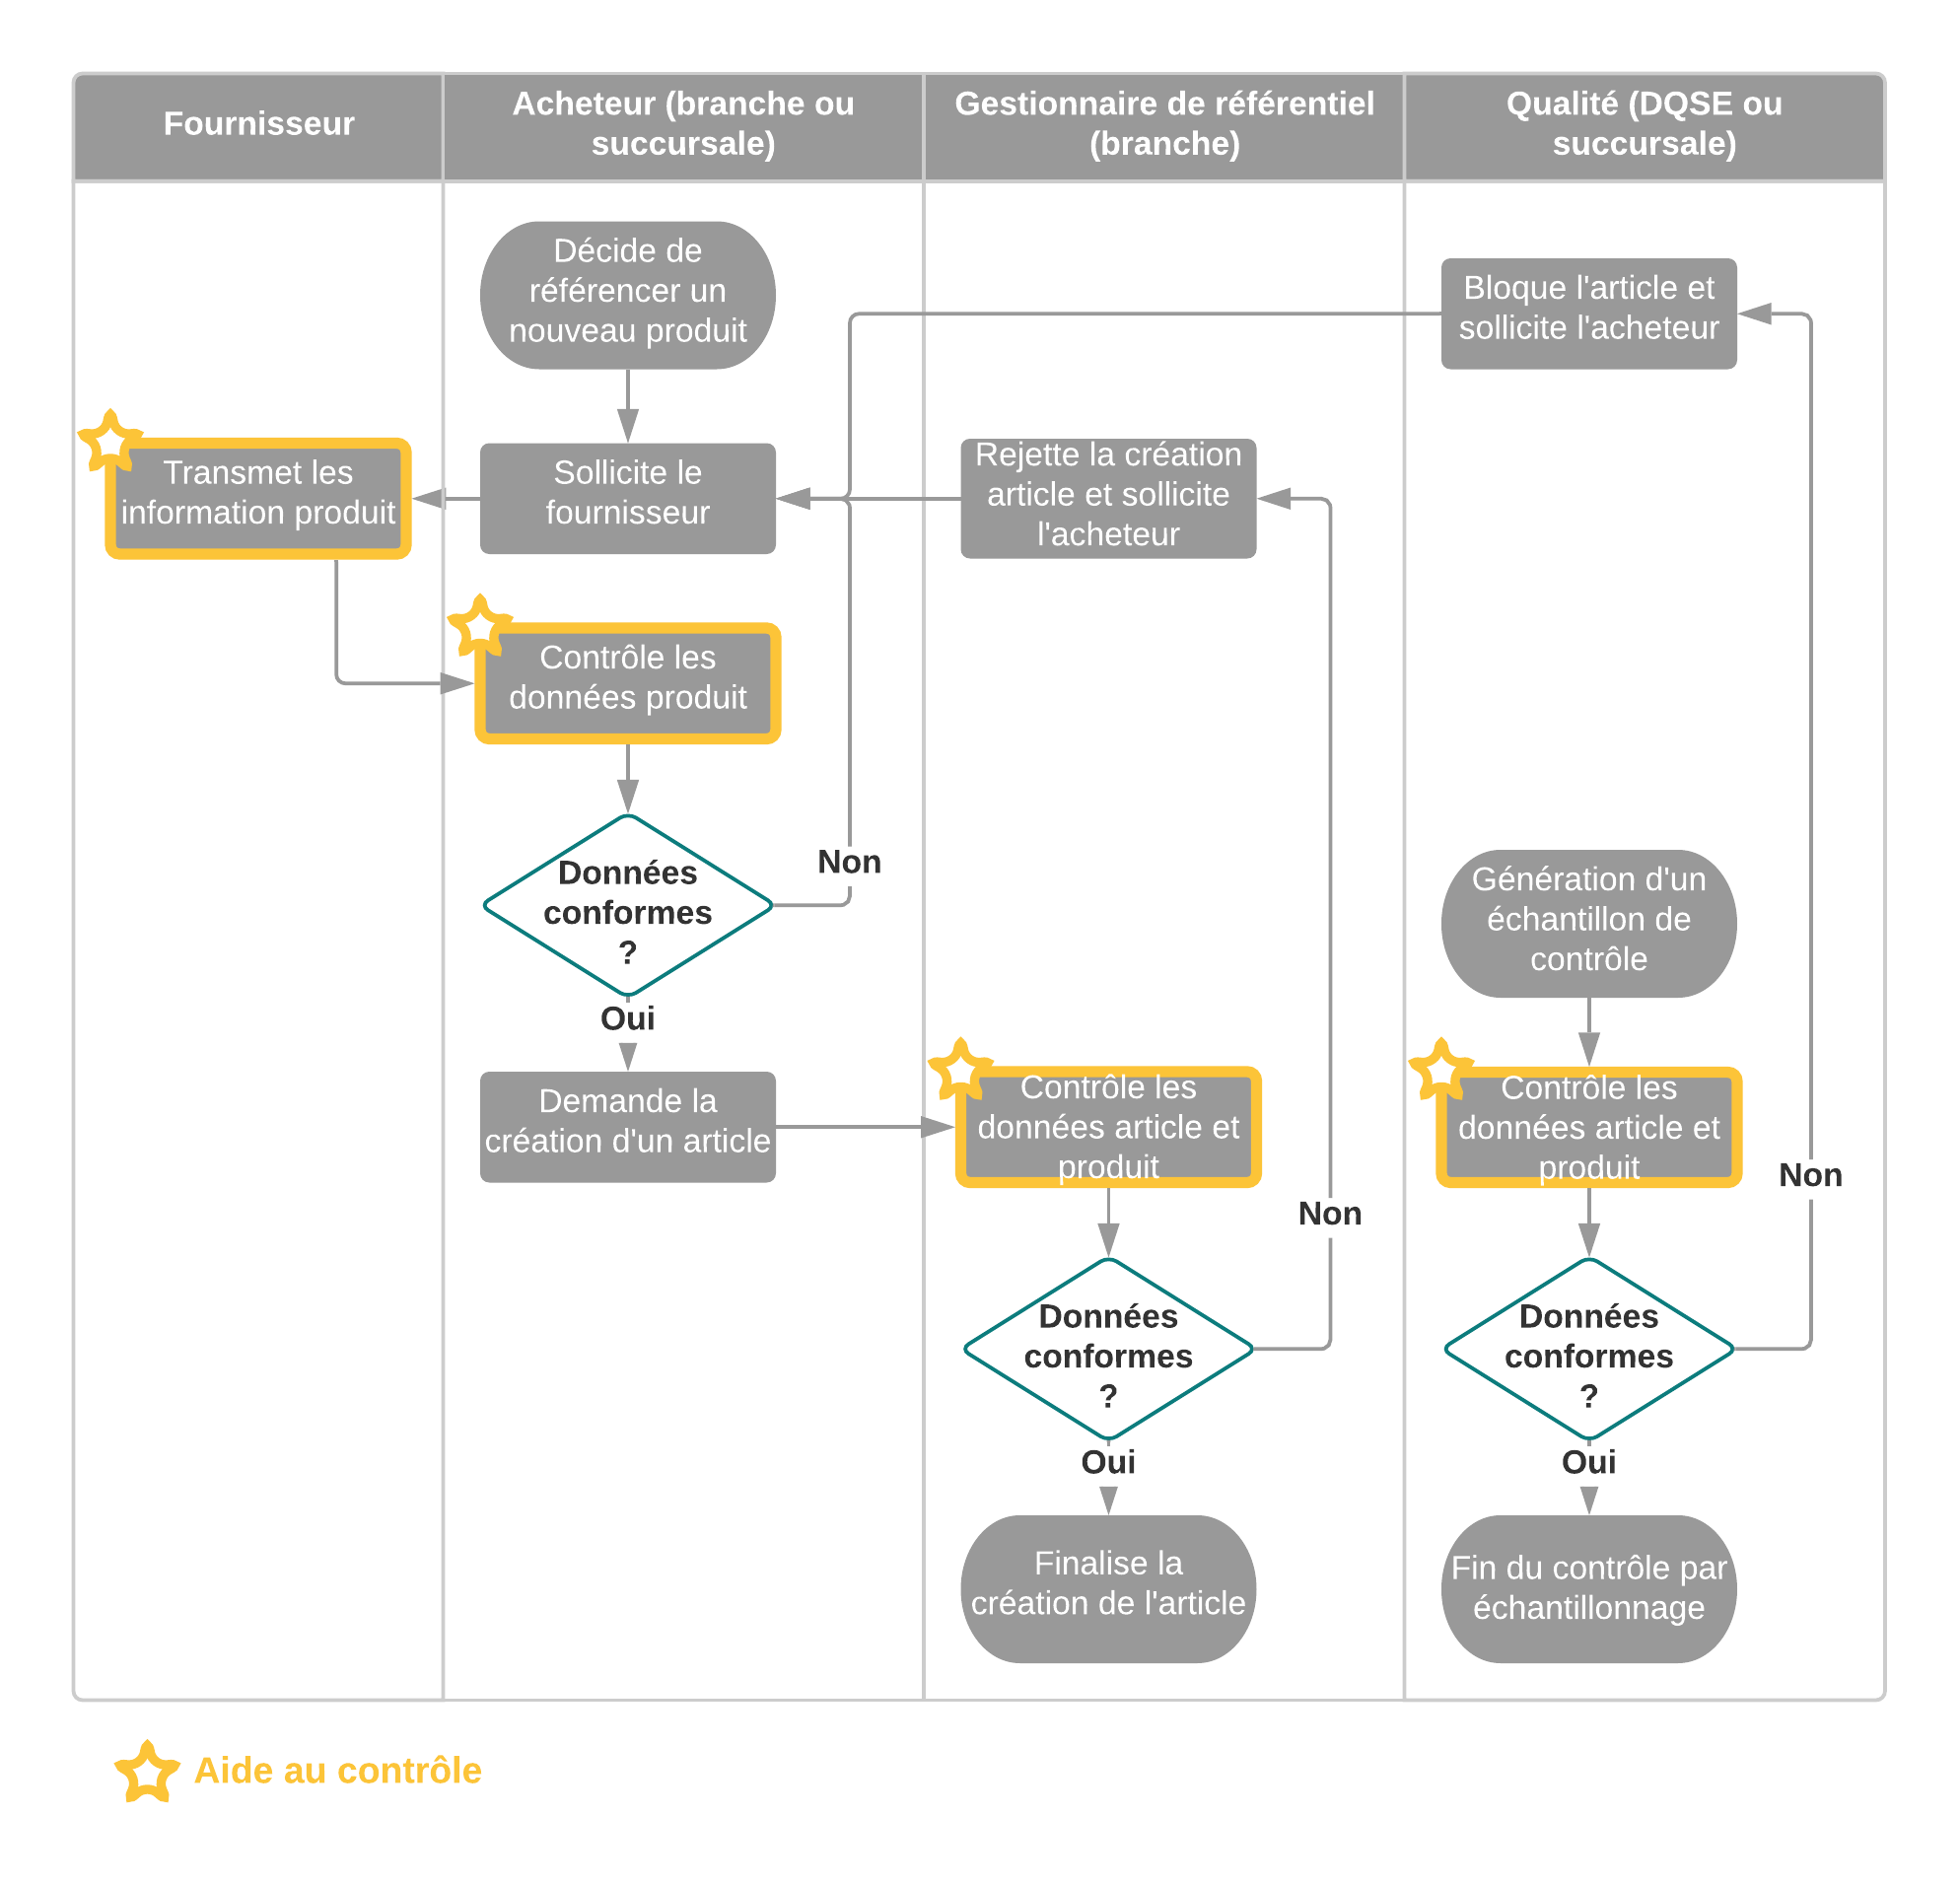
\includegraphics[width=0.9\linewidth]{img/Processus_de_creation_article_avec_aide_au_controle.png}
            \end{center}
            \caption{\'{E}tapes du processus article pouvant être améliorées}
            \label{fig:processus_article_aide_ctrle}
        \end{figure}    

            \subsection{Le contrôle à la saisie fournisseur}
            Si on déclenche un contrôle au moment où le fournisseur soumet les données et qu'on l'alerte en cas d'incohérence, on peut dès le début du processus éviter une erreur.
            L'avantage d'avoir une identification des problèmes aussi tôt est qu'on économise immédiatement au moins une étape de contrôle des données.

            \subsection{L'aide aux vérifications Pomona}
            Lors des contrôles inclus au sein du processus, on pourrait mettre en évidence les incohérences détectées entre pièces jointes et données à contrôler.
            Cela permettrait de fiabiliser les étapes de contrôle, et éviter qu'une erreur soit détectée tardivement (par les gestionnaires de référentiel ou les ingénieurs qualité).
            C'est d'autant plus intéressant que la première étape de contrôle est faite par les acheteurs.
            Dans la mesure où c'est une tâche administrative qui n'est pas dans leur c{\oe}ur de métier, elle est souvent effectuée rapidement et est peu efficace.

            \subsection{Les contrôles en masse asynchrones}
            Enfin, il pourrait être pertinent de faire tourner de manière asynchrone des contrôles de qualité de données sur l'ensemble de la base.
            Il pourrait sembler inutile d'effectuer cette tâche alors qu'on a une validation des données par l'application (contrôles \og informatiques \fg) et par des contrôleurs humains.
            Néanmoins, il arrive fréquemment que des changements de règles de gestion informatiques ou métier soit mis en place, sans que les données soient ensuite remises à jour.
            Par exemple, les mentions des traces d'allergènes dans les ingrédients était par le passé retirées des listes d'ingrédients, alors qu'elle sont aujourd'hui incluses. 
            Mais aucun chantier de remise à niveau de l'historique n'a été entrepris au moment du changement de règle, d'où des données qui ne sont pas alignées avec les règles de gestion.

    \chapter{Le choix du cas d'usage}

        \section{\'{E}tiquettes contre fiches techniques}

            \subsection{La représentation dominante des fiches techniques}
            
            Les pièces jointes utilisées lors des contrôles métier pour la vérification des données produit sont les fiches techniques fournisseur et les étiquettes.
            Or, les étiquettes sont moins représentées que les fiches techniques dans le PIM (cf. \reftable{tbl:attached_files_counts}).
            
            \subsection{L'extraction de données textuelles}

            Comme cela a été décrit à la section \mref{etiquettes_produit} Les étiquettes sont des pièces jointes au format pdf, mais qui peuvent être générées de multiples façons : 
            \begin{itemize}
                \item issues d'un logiciel graphique pour la constitution du applat du packaging
                \item construites à partir d'une ou plusieurs photos insérées dans outil de traitement de texte
                \item \dots
            \end{itemize}
            Les textes présents dans ces pdf se présentent donc parfois sous forme de textes extractibles par des bibliothèques de pdf mining, soit sous forme d'images qui nécessitent alors des fonctionnalités d'OCR (Optical Character Recognition~\cite{OCR_wiki}).
            Le taux de pièces jointes avec des textes extractibles a été présenté à la \reftable{tbl:empty_attached_files} ; pour mémoire seul un tiers des étiquettes ont un contenu exploitable par les outils de pdfmining.
            De plus, l'orientation des textes peut parfois faire l'objet d'une rotation (cf. l'étiquette des lentilles en annexe \mref{ex:ET_lentilles}), voire n'être pas toujours la même selon les faces de l'emballage (cf. l'étiquette de la panna cotta, en annexe \mref{ex:ET_pannacotta}).
            Ces contraintes, bien que surmontables, imposent des travaux qui n'auraient pas d'intérêt dans le cadre de ce mémoire.

            \emphbox{On va donc dans un premier temps travailler avec les fiches techniques plutôt qu'avec les étiquettes}

        
        \section{Impossibilité de produire des templates pour l'exploitation de ces documents}

        Chaque fournisseur décide du format des fiches techniques qu'il souhaite produire.
        On a donc beaucoup de formats différents, à peu de choses près on a un format par fournisseur.
        On pourrait imaginer développer un outil qui sur la base d'un template permet d'extraire de manière fiable le contenu de documents qui ont toujours le même format (cela se fait par exemple pour les commandes clients reçues par mail).
        L'établissement d'un \og traducteur \fg de documents de ce type représente une charge d'une dizaine de jours de travail par format de fichier.
        Le Pareto des produits par fournisseur présenté à la \reffig{fig:rappel_pdt_par_frn} montre qu'il ne serait pas économiquement pertinent de construire ce genre d'outil (10 templates ne permettraient de couvrir que 3000 produits, et le gain marginal ne cesserait de diminuer ensuite).
        On n'approche pas du seuil de rentabilité requis. 
        En comparaison, les outils de parsing des commandes mail permettent de traiter plus de 20 000 postes de commandes par jour, avec moins de 5 templates.

        \emphbox{Une approche traditionnelle d'extraction de données depuis des documents pdf ne pourra pas être appliquée pour ce cas d'usage}

        \section{Quelles données ?}

            \subsection{Les principales données et leur mode de présentation dans les fiches techniques}
            Les données que l'on souhaite récupérer sont globalement de 4 types : 
            \begin{itemize}
                \item données de composition : listes d'ingrédients
                \item données de composition : allergènes
                \item données nutritionnelles
                \item données logistiques
            \end{itemize}

            Comme vu dans la section \mref{fiches_techniques}, parmi les données présentes dans les fiches techniques, seule la liste d'ingrédients se présente quasiment toujours sous la forme d'un texte brut (par opposition à un affichage au sein d'un tableau).
            La représentation des données nutritionnelles se fait régulièrement sous forme de tableau, les données logistiques également (cf. les exemples de fiches techniques présentées en annexe, à partir de \mref{ex:FT_sel}).
        
            \subsection{L'identification d'une liste d'ingrédient par son contenu}

            Il est possible de dire si un texte est une liste d'ingrédients, juste en lisant ce texte.
            Il s'agit souvent d'une énumération d'ingrédients individuels (cf. la section \mref{listes_ingredients}).
            Même sortie de son contexte, il est en général faisable pour un humain d'identifier comme telle une liste d'ingrédients.
            Par exemple : 
            \begin{quotation}
                Huile de colza (70.45 \%), jaunes d’oeufs (6.2 \%), purée de tomates, eau, vinaigre, câpres (2.8 \%) (câpres, eau, sel),cornichons (2.8 \%) (cornichons, vinaigre, sel), sucre, sel,amidon modifié, acidifiant : lucono-delta-lactone, conser-vateur : sorbate de potassium, antioxydant : E385 (74mg/kg), épice, arôme naturel aneth
            \end{quotation}
            est de toute évidence une liste d'ingrédients.

            \`{A} l'inverse, les autres grands types d'information nécessitent du contexte dans le document.
            Par exemple, \og 14g \fg peut être une quantité de glucides, de lipides, le poids d'une pièce unitaire, \dots
            
            \emphbox{L'identification de listes d'ingrédients pourrait se faire sans avoir à construire de fonctionnalités s'appuyant sur le contexte au sein du document}

        \section{Quels produits ?}
        
        Pour des raisons d'accessibilité de la donnée, on travaillera sur les produits de la branche \'{E}piSaveurs. 
        Il est de toute façon prévu de déployer le PIM sur l'ensemble des autres branches du groupe, on pourra adresser leurs produits à ce moment-là.
        La notion d'ingrédients n'a pas de sens pour les produits d'hygiène (cf. section \mref{produits_nonal} sur les produits non-alimentaires), mais existe pour les produits de chimie.
        Comme les ingrédients des produits alimentaires sont en général différents des produits de chimie, on se limitera d'abord aux premiers.
        Enfin, la réglementation étant moins stricte pour les boissons alcoolisées sur le sujet spécifique de l'étiquetage de la composition, on ne les prendra pas non plus en compte dans ce mémoire.

        \section{Conclusion quant au choix du cas d'usage}

        \emphbox{Au vu des différentes contraintes listées dans cette partie, on s'attachera à extraire \emph{les listes d'ingrédients} des produits \emph{alimentaires} de la branche \emph{EpiSaveurs} (épicerie et boissons non alcoolisées) depuis \emph{les fiches techniques fournisseur}, en se basant sur \emph{le contenu textuel} de ces documents.}